\documentclass{beamer}
\usetheme{default}

\usepackage{amsmath,amssymb,mathrsfs,bm}
\usepackage{anyfontsize}
\usepackage{unicode-math}
\unimathsetup{math-style=ISO, bold-style=ISO, mathrm=sym}
\setmathfont{XITS Math}
\usepackage{fontspec}
\setsansfont{Linux Biolinum O}
\setmonofont{JetBrains Mono NL}
\AtBeginDocument{
  \let\uglyepsilon\epsilon
  \renewcommand\epsilon{\varepsilon}
}
\AtBeginDocument{
  \let\uglymathsf\mathsf
  \renewcommand\mathsf{\symsf}
}
\renewcommand{\bm}{\symbf}

\usepackage[fontset=none]{ctex}
\setCJKmainfont{宋体}[BoldFont=Noto Serif CJK SC Bold]
\setCJKsansfont{Noto Sans CJK SC}[RawFeature=+fwid]
\setCJKmonofont{Noto Sans Mono CJK SC}[RawFeature=+fwid]
\newCJKfontfamily\songti{宋体}[BoldFont=Noto Serif CJK SC Bold]
\newCJKfontfamily\heiti{Noto Sans CJK SC}[RawFeature=+fwid]
\newCJKfontfamily\kaishu{楷体}
\newCJKfontfamily\fangsong{仿宋}
\newCJKfontfamily\lishu{方正隶书简体}
\newCJKfontfamily\yahei{Noto Sans CJK SC}[RawFeature=+fwid]
\newCJKfontfamily\youyuan{方正兰亭圆简体}

\usepackage{color}
\usepackage{graphicx,caption,subcaption}
\usepackage{hyperref}
\hypersetup{
    colorlinks=true,
    linkcolor=blue,
    filecolor=green,
    urlcolor=cyan,
    citecolor=cyan,
}

\usepackage{listings}
\lstset{
    language=Python,
    basicstyle=\ttfamily\tiny,
    aboveskip={1.0\baselineskip},
    belowskip={1.0\baselineskip},
    columns=fixed,
    extendedchars=true,
    breaklines=true,
    tabsize=4,
    prebreak=\raisebox{0ex}[0ex][0ex]{\ensuremath{\hookleftarrow}},
    frame=lines,
    showtabs=false,
    showspaces=false,
    showstringspaces=false,
    keywordstyle=\color[rgb]{0,0.5,0},
    commentstyle=\color[rgb]{0.5,0,0},
    stringstyle=\color[rgb]{1,0,0},
    numbers=left,
    numberstyle=\tiny\ttfamily,
    stepnumber=1,
    numbersep=12pt,
    captionpos=t,
    escapeinside={\%*}{*)}
}

\title{我的Beamer模板}
\author{北京大学\ \ 张植竣}
\date{\today}

\begin{document}

\begin{frame}[plain]
    \maketitle
\end{frame}

\begin{frame}{Frame Title 1}
    \begin{center}
        赴戍登程口占示家人二首（其二）
        \medskip

        \fangsong{【清】林则徐}
        \bigskip

        \kaishu{
        力微任重久神疲，再竭衰庸定不支。

        苟利国家生死以，岂因祸福避趋之！

        谪居正是君恩厚，养拙刚于戍卒宜。

        戏与山妻谈故事，试吟断送老头皮。
        }
    \end{center}
\end{frame}

\begin{frame}{Frame Title 2}
    \[
    \iiint \nabla\cdot\symbf{A}\,\symrm{d}V = \oiint \symbf{A}\,\symrm{d}\symbf{S}
    \]
    \begin{align*}
        [q,p]_{Q,P}
        &= \frac{\partial q}{\partial Q}\cdot\frac{\partial p}{\partial P} - \frac{\partial q}{\partial P}\cdot\frac{\partial p}{\partial Q} \\
        &= \left(-\frac{\sqrt{1-P^2\symrm{e}^{2Q}}}{\symrm{e}^Q} - \frac{P^2\symrm{e}^Q}{\sqrt{1-P^2\symrm{e}^{2Q}}}\right)\cdot\left(\frac{-\symrm{e}^Q}{\sqrt{1-P^2\symrm{e}^{2Q}}}\right) - \\
        &\quad\left(\frac{-P\symrm{e}^Q}{\sqrt{1-P^2\symrm{e}^{2Q}}}\right)\cdot\left(\frac{-P\symrm{e}^Q}{\sqrt{1-P^2\symrm{e}^{2Q}}}\right) \\
        &= 1 + \frac{P^2\symrm{e}^{2Q}}{1-P^2\symrm{e}^{2Q}} - \frac{P^2\symrm{e}^{2Q}}{1-P^2\symrm{e}^{2Q}} \\
        &= 1
    \end{align*}
\end{frame}

\begin{frame}{Frame Title 3}
    \begin{equation}
    D_n = \frac{2}{l}\int_0^l\frac{2blx^3-abx^4}{12a^2}\sin\frac{n\pi}{2l}x \,\mathrm{d}x = \left\{
    \begin{aligned}
        0\qquad &,\quad n = 2k \\
        -\frac{8bl^4}{a^2 \pi^5 n^5}&,\quad n = 2k + 1
    \end{aligned}
    \right.
    \end{equation}
    \begin{equation}
    w(x,0) = 0,\qquad \left.\frac{\partial w}{\partial t}\right|_{t=0} = -\left.\frac{\partial v}{\partial t}\right|_{t=0} = -\frac{Aa\sin\left(\dfrac{\omega x}{a}\right)}{ES\cos\left(\dfrac{\omega l}{a}\right)}
    \end{equation}
\end{frame}

\begin{frame}{Frame Title 4}
    \begin{itemize}
        \item[\bullet] 我能吞下玻璃而不伤身体
        \begin{itemize}
            \item[\bullet][1.] \songti{我能吞下玻璃而不伤身体。，、——：；‘“恭喜发财”’！？}

            \item[\bullet][2.] \kaishu{我能吞下玻璃而不伤身体。，、——：；‘“恭喜发财”’！？}

            \item[\bullet][3.] \fangsong{我能吞下玻璃而不伤身体。，、——：；‘“恭喜发财”’！？}

            \item[\bullet][4.] \heiti{我能吞下玻璃而不伤身体。，、\symbol{"2E3A}：；‘“恭喜发财”’！？}

            \item[\bullet][5.] \lishu{我能吞下玻璃而不伤身体。，、——：；‘“恭喜发财”’！？}
        \end{itemize}

        \item[\bullet] \href{https://www.php.net/}{PHP}是世界上最好的语言

        \item[\bullet] \songti{欢迎来到\textbf{\textcolor[RGB]{139,0,18}{北京大学}}物理学院！}
    \end{itemize}
\end{frame}

\begin{frame}{Frame Title 5}
    \begin{figure}[ht]
        \centering
        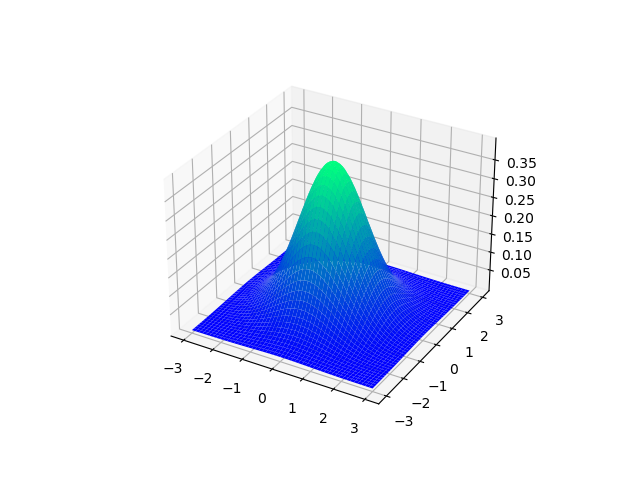
\includegraphics[width=0.6\textwidth]{Template_Picture.png}
        \caption*{Template Picture}
    \end{figure}
\end{frame}

\begin{frame}{Frame Title 6}
    模板代码：
    \lstinputlisting{Template_Code.py}
\end{frame}

\begin{frame}{Frame Title 8}
    Itemize example: \pause
    \begin{itemize}
        \item[\bullet] Ceasar said: “Veni, Vidi, Vici.” \pause
        \item[\bullet] Karl Marx said: “The history of all hitherto existing society is the history of class struggles.” \pause
    \end{itemize}
    Enumerate example: \pause
    \begin{enumerate}
        \item[\bullet] \LaTeX{} beamer is powerful. \pause
        \item[\bullet] \LaTeX{} beamer is beautiful. \pause
    \end{enumerate}
\end{frame}

\begin{frame}{Frame Title 8}
    \begin{columns}
        \begin{column}{0.5\linewidth}
            \colorbox{red}{Fourier变换}
            \[
            F(\omega) = \frac{1}{\sqrt{2\pi}}\int_{-\infty}^{\infty}f(t)\mathrm{e}^{-i\omega t}\,\mathrm{d}t
            \]
        \end{column}
        \begin{column}{0.5\linewidth}
            \colorbox{yellow}{Fourier逆变换}
            \[
            f(t) = \frac{1}{\sqrt{2\pi}}\int_{-\infty}^{\infty}F(\omega)\mathrm{e}^{i\omega t}\,\mathrm{d}\omega
            \]
        \end{column}
    \end{columns}
\end{frame}

\begin{frame}
    \begin{center}
        \Huge 谢谢大家！
    \end{center}
\end{frame}

\end{document}
